\documentclass[./main.tex]{subfiles}

\begin{document}
\section{Comparison}

The algorithms were compared on all instances of the wareshouse allocation problem.
Every instance was solved 11 times for 8 different amounts of evaluation calls, starting from $1000$ and ending by $5000000$ calls.
These three algorithms were run in parallel.

In the following subsections are presented plots comparing these three algorithms in terms of quality of solution as a function of number of evaluation calls.

The plots contains box plot for each batch. Boxplots belonging to individual algorithms have connected means to better visualize, when each algorithm gets better than the others.

On $y$ axis are plotted only fitness function values excluding constraint violations for infeasible solutions.
Algorithms find valid solutions really quickly, so for plotted evaluation call limits, the common fitness function and fitness function considering violations have the same value.

What those charts do not include is runtime of algorithms, which will be described in conclusion.

\newpage
\subsection{wl\_16\_1}
On this instance, the local search algorithm outperforms both basic evolution algorithm and mine specialized memetic algorithm with evolution algorithm being better than the memetic one.
This can be caused by the greedy initialization, or that the local search is more likely to shift to more promising areas due to more random trials, while the other two algorithms try to combine already found solutions and the pure randomization isn't so frequent.
Quite interesting is, that the memetic algorithm struggles against the evolutionary one.
This is probably caused by evaluation calls "wasted" on local search, so it does not perform as many population generations.
However, as opposed to the other two, the memetic algorithm decreases monotically while tightening the confidence bounds, so even though the found solution is not as good, it is unlikely, that it will get stuck in some worse.
That cannot be said about the two other as their confidence bounds are huge and not with improving trend.
\begin{figure}[ht]
    \centering
    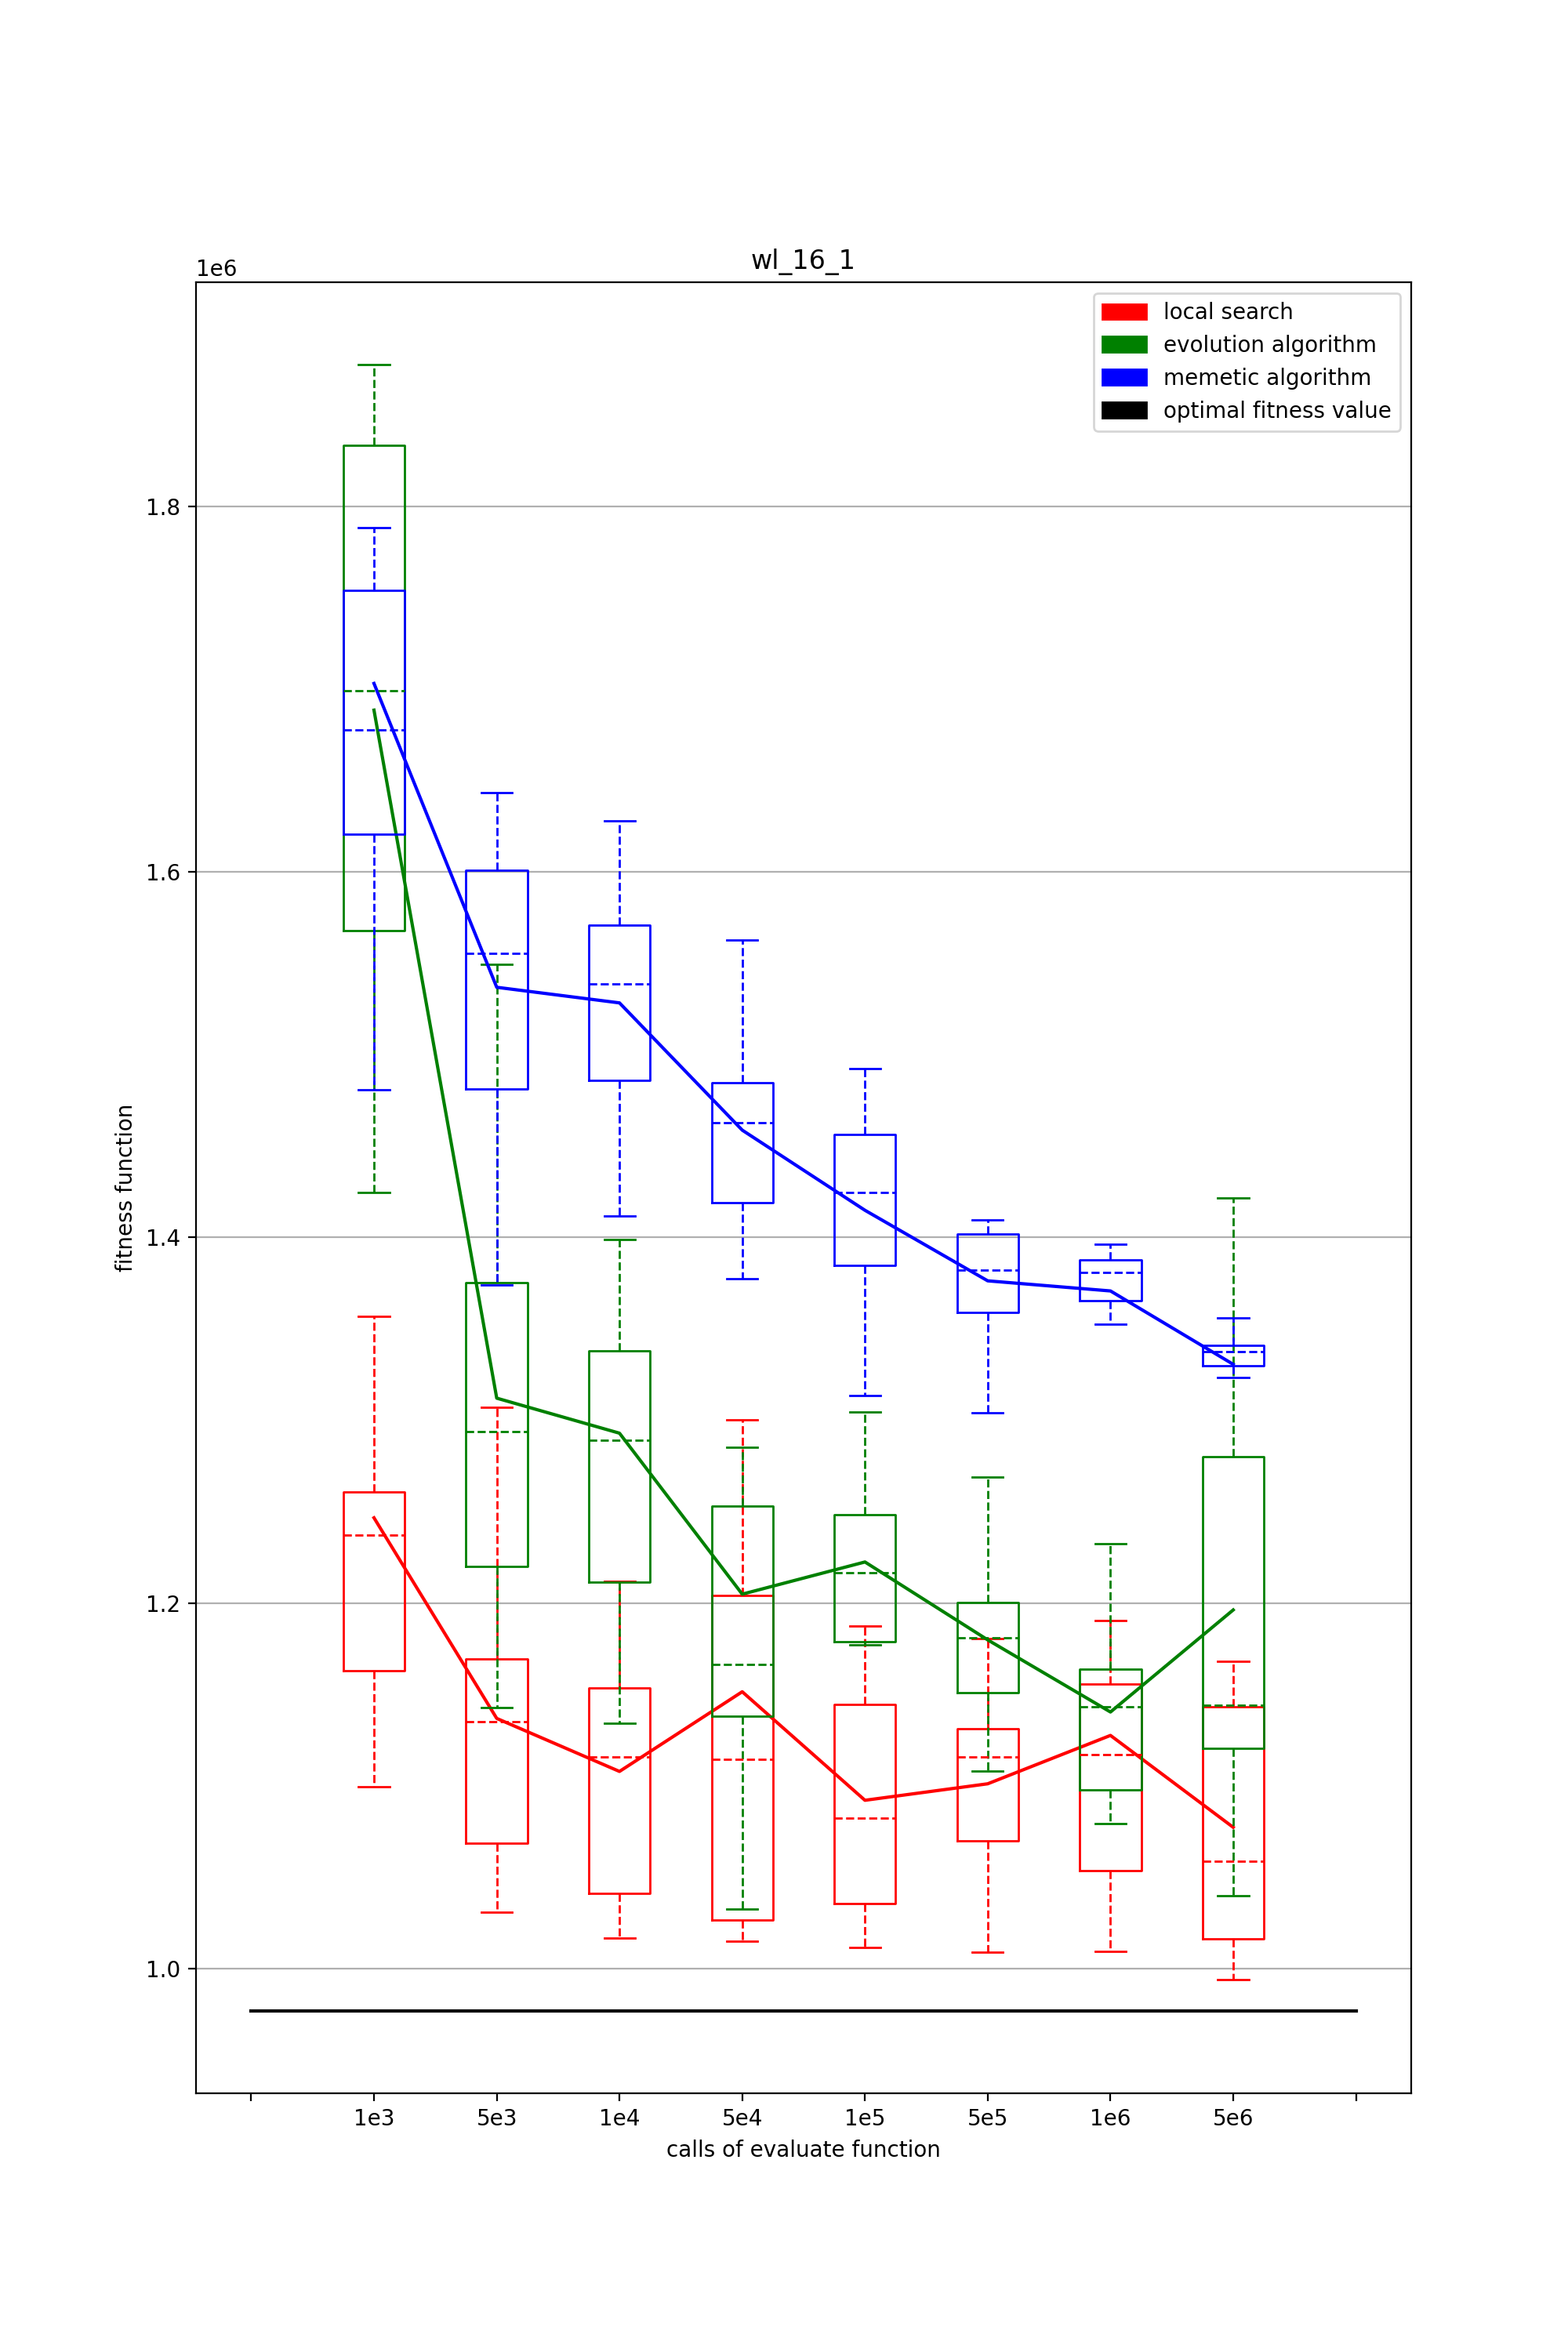
\includegraphics[width=0.6\linewidth]{wl_16_1.png}
    \caption{Comparison of algorithms on wl\_16\_1 instance}
\end{figure}

\newpage
\subsection{wl\_25\_2}
This instance is easy, so all algorithms find really good solutions quickly.
The memetic algorithm always finds the same solution and that will probably be caused by the greedily initialized candidate, which will get him stuck in some local optima and the mutation pressure isn't as great as in local search.
On the other hand, the evolutionary algorithm oscilates quite a bit, so the best solution isn't guranteed to be reached every time.
Local search finds really good solution after approximately 1000 random trials and then is not able to improve further.
Also, the evolutionary algorithm needs a lot of evaluations to combine the population so the solutions are good. The random initialization obviously creates really bad solutions.
\begin{figure}[ht]
    \centering
    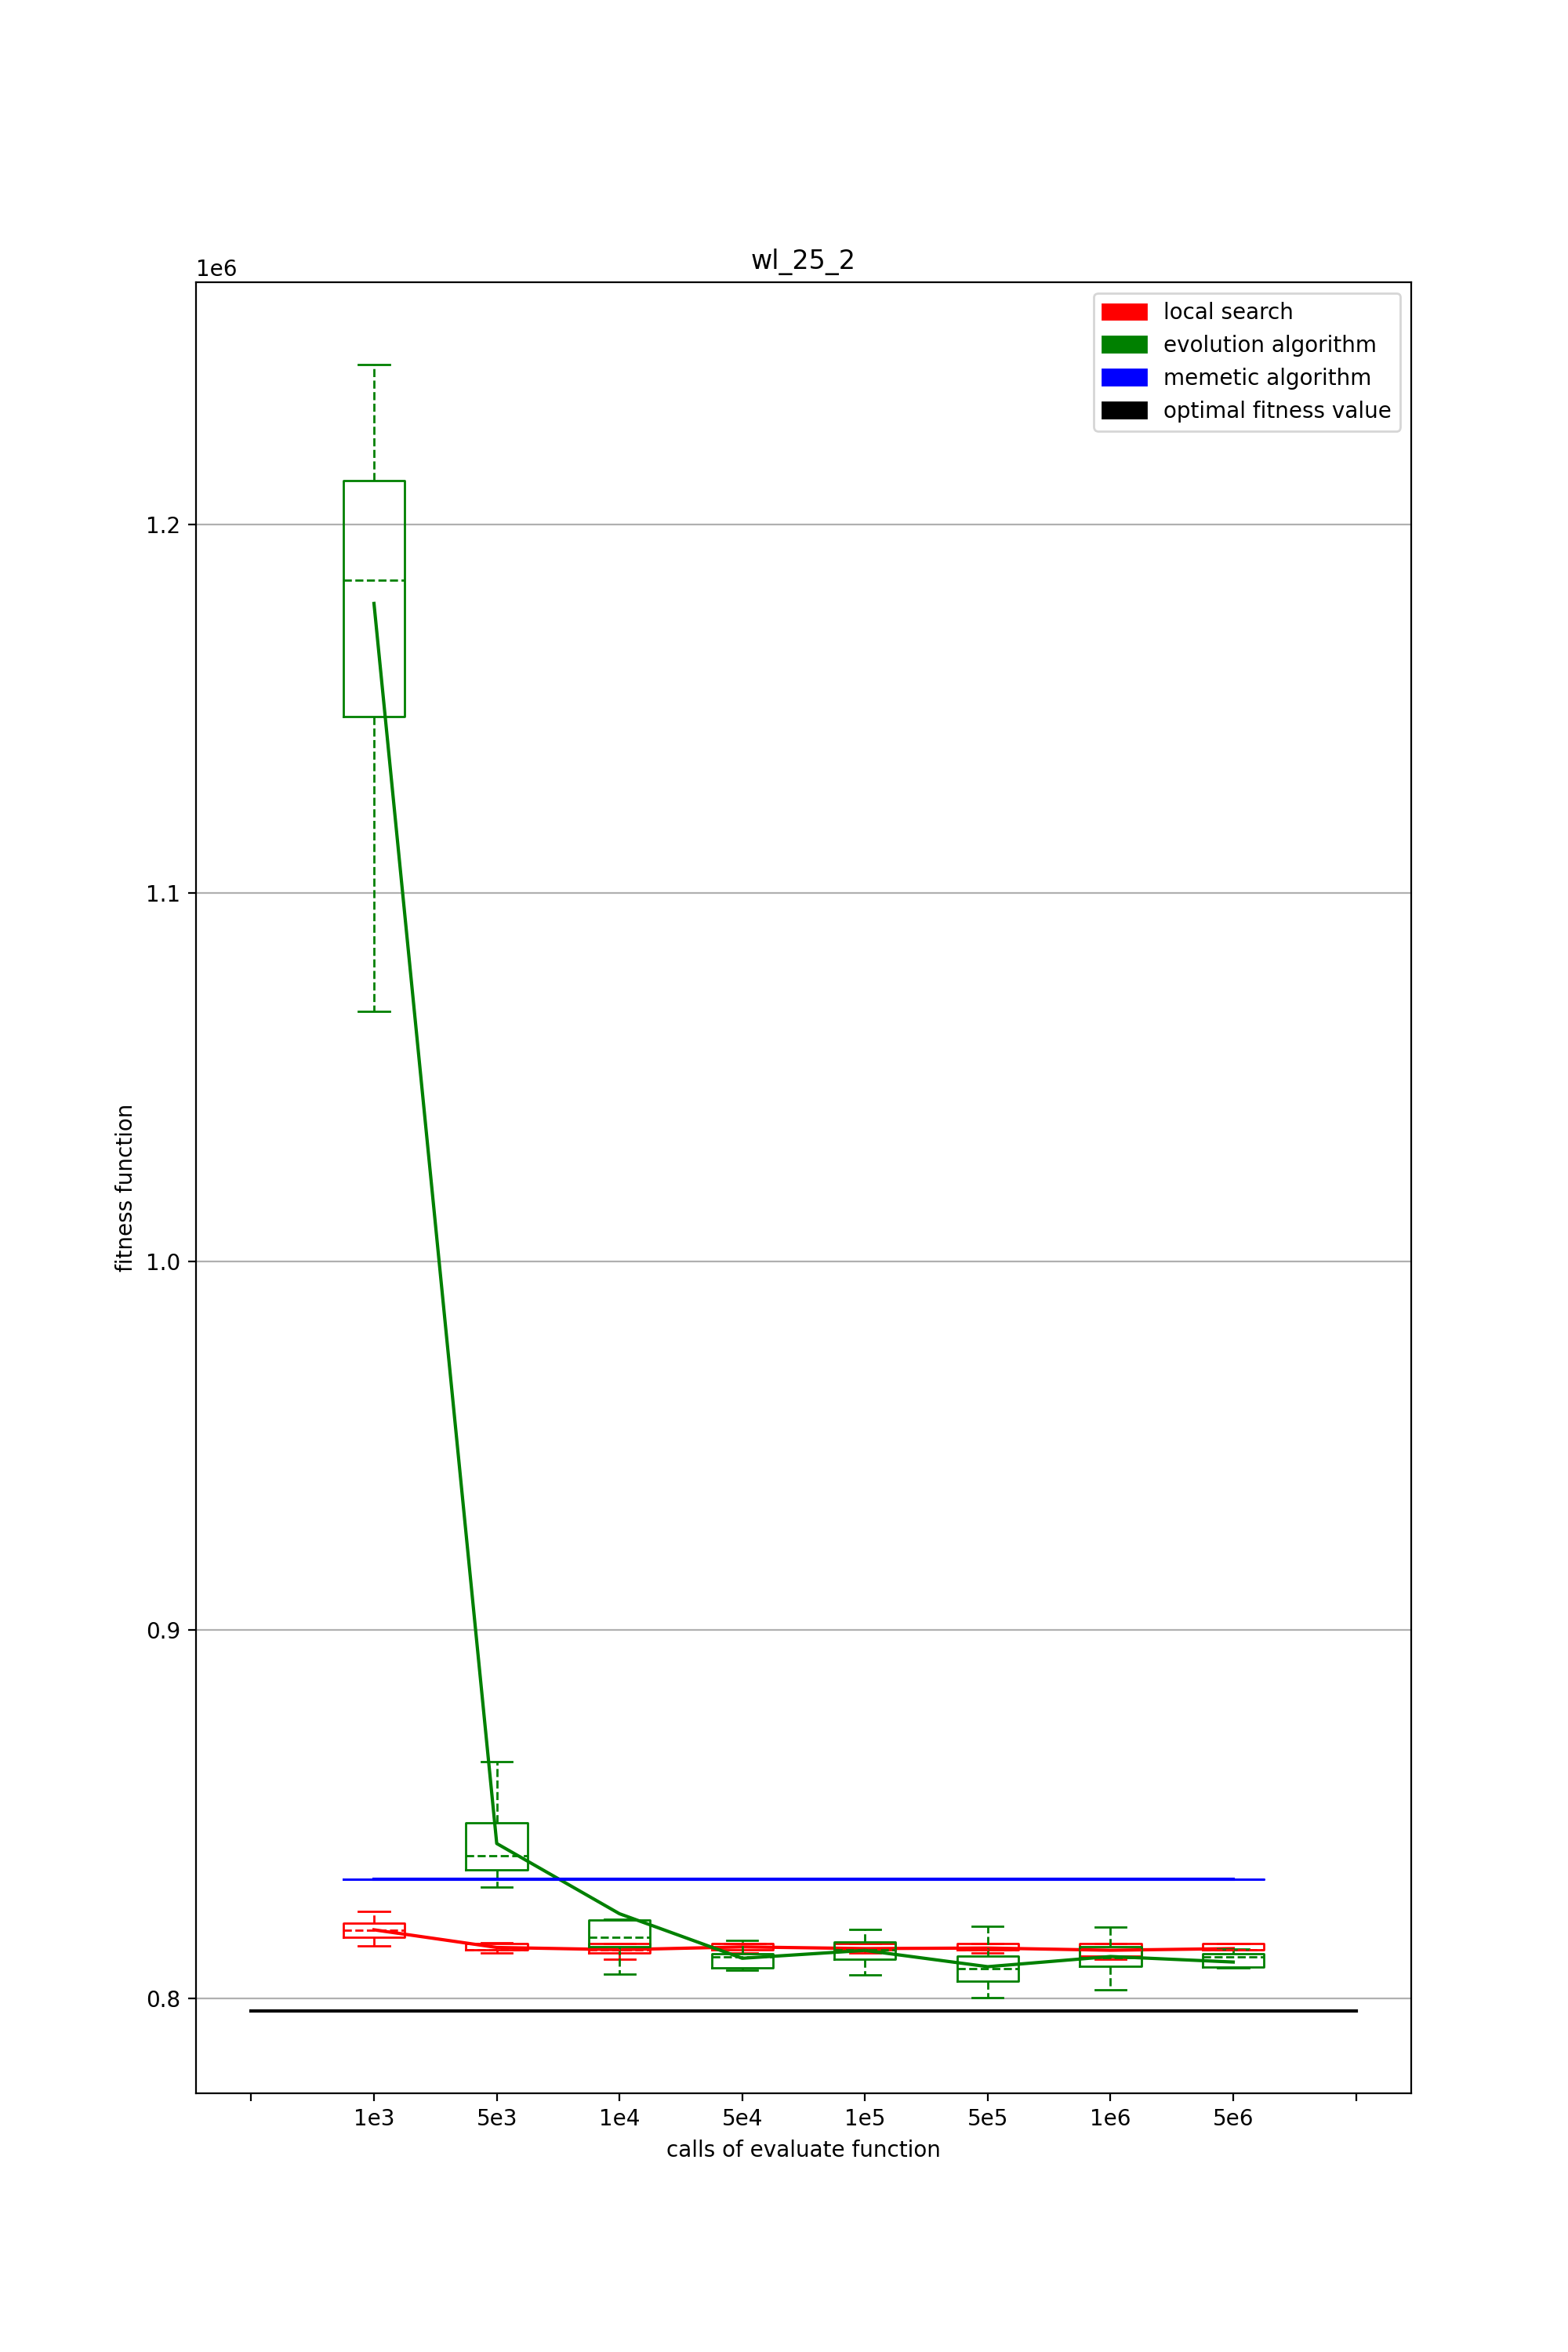
\includegraphics[width=0.6\linewidth]{wl_25_2.png}
    \caption{Comparison of algorithms on wl\_25\_2 instance}
\end{figure}

\newpage
\subsection{wl\_50\_1}
Situation on this instance is almost exactly the same as in previous instance.
It is really easy, so the power of the memetic algorithm doesn't show in comparison.
Maybe, it would be suitable to perform local search also before the breeding phase in the memetic algorithm, so there would be possibility to get to another areas and not get stuck.
\begin{figure}[ht]
    \centering
    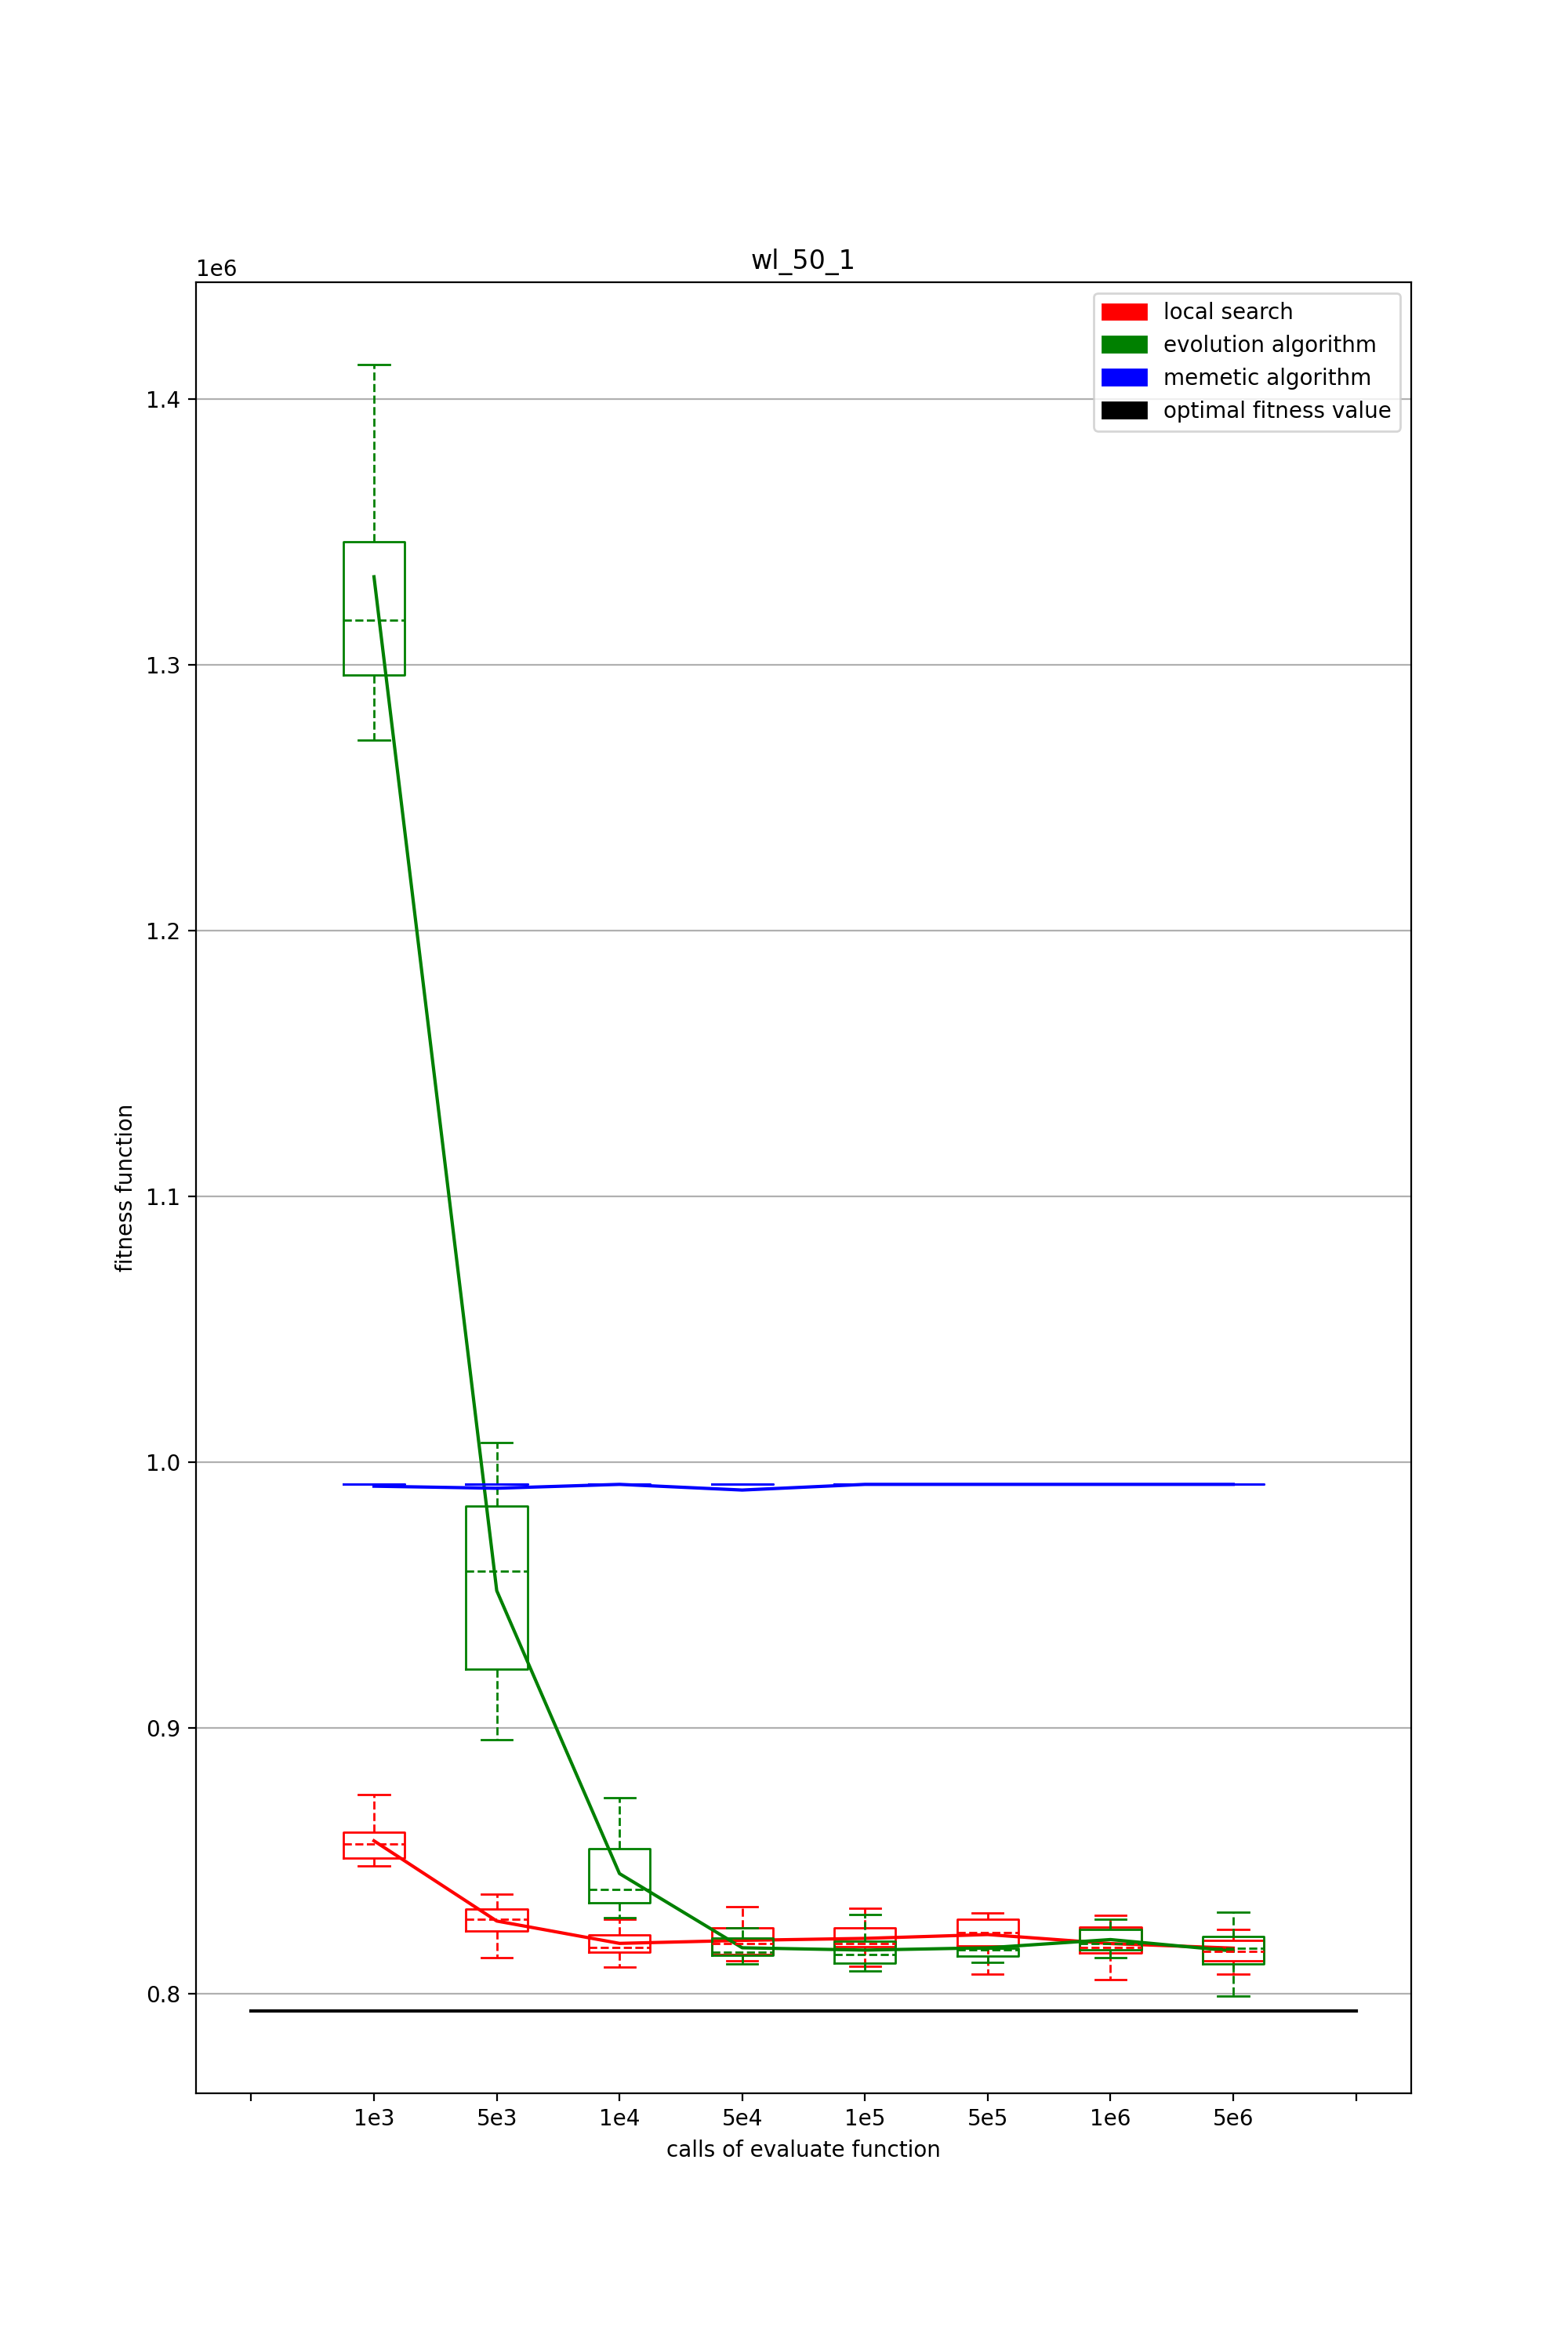
\includegraphics[width=0.6\linewidth]{wl_50_1.png}
    \caption{Comparison of algorithms on wl\_50\_1 instance}
\end{figure}

\newpage
\subsection{wl\_100\_4}
This instance is where the situation changes.
It is probably much harder and the local search simply does not have a chance to improve much from the greedy candidate.
The evolution algorithm improves a bit, but it only gets stuck in a better solution.
The best is the memetic one, possibly because it has more mutation power than the evolution algorithm and it is able to jump to more promising areas, where the evolution starts working again and starts finding better and better solutions.
\begin{figure}[ht]
    \centering
    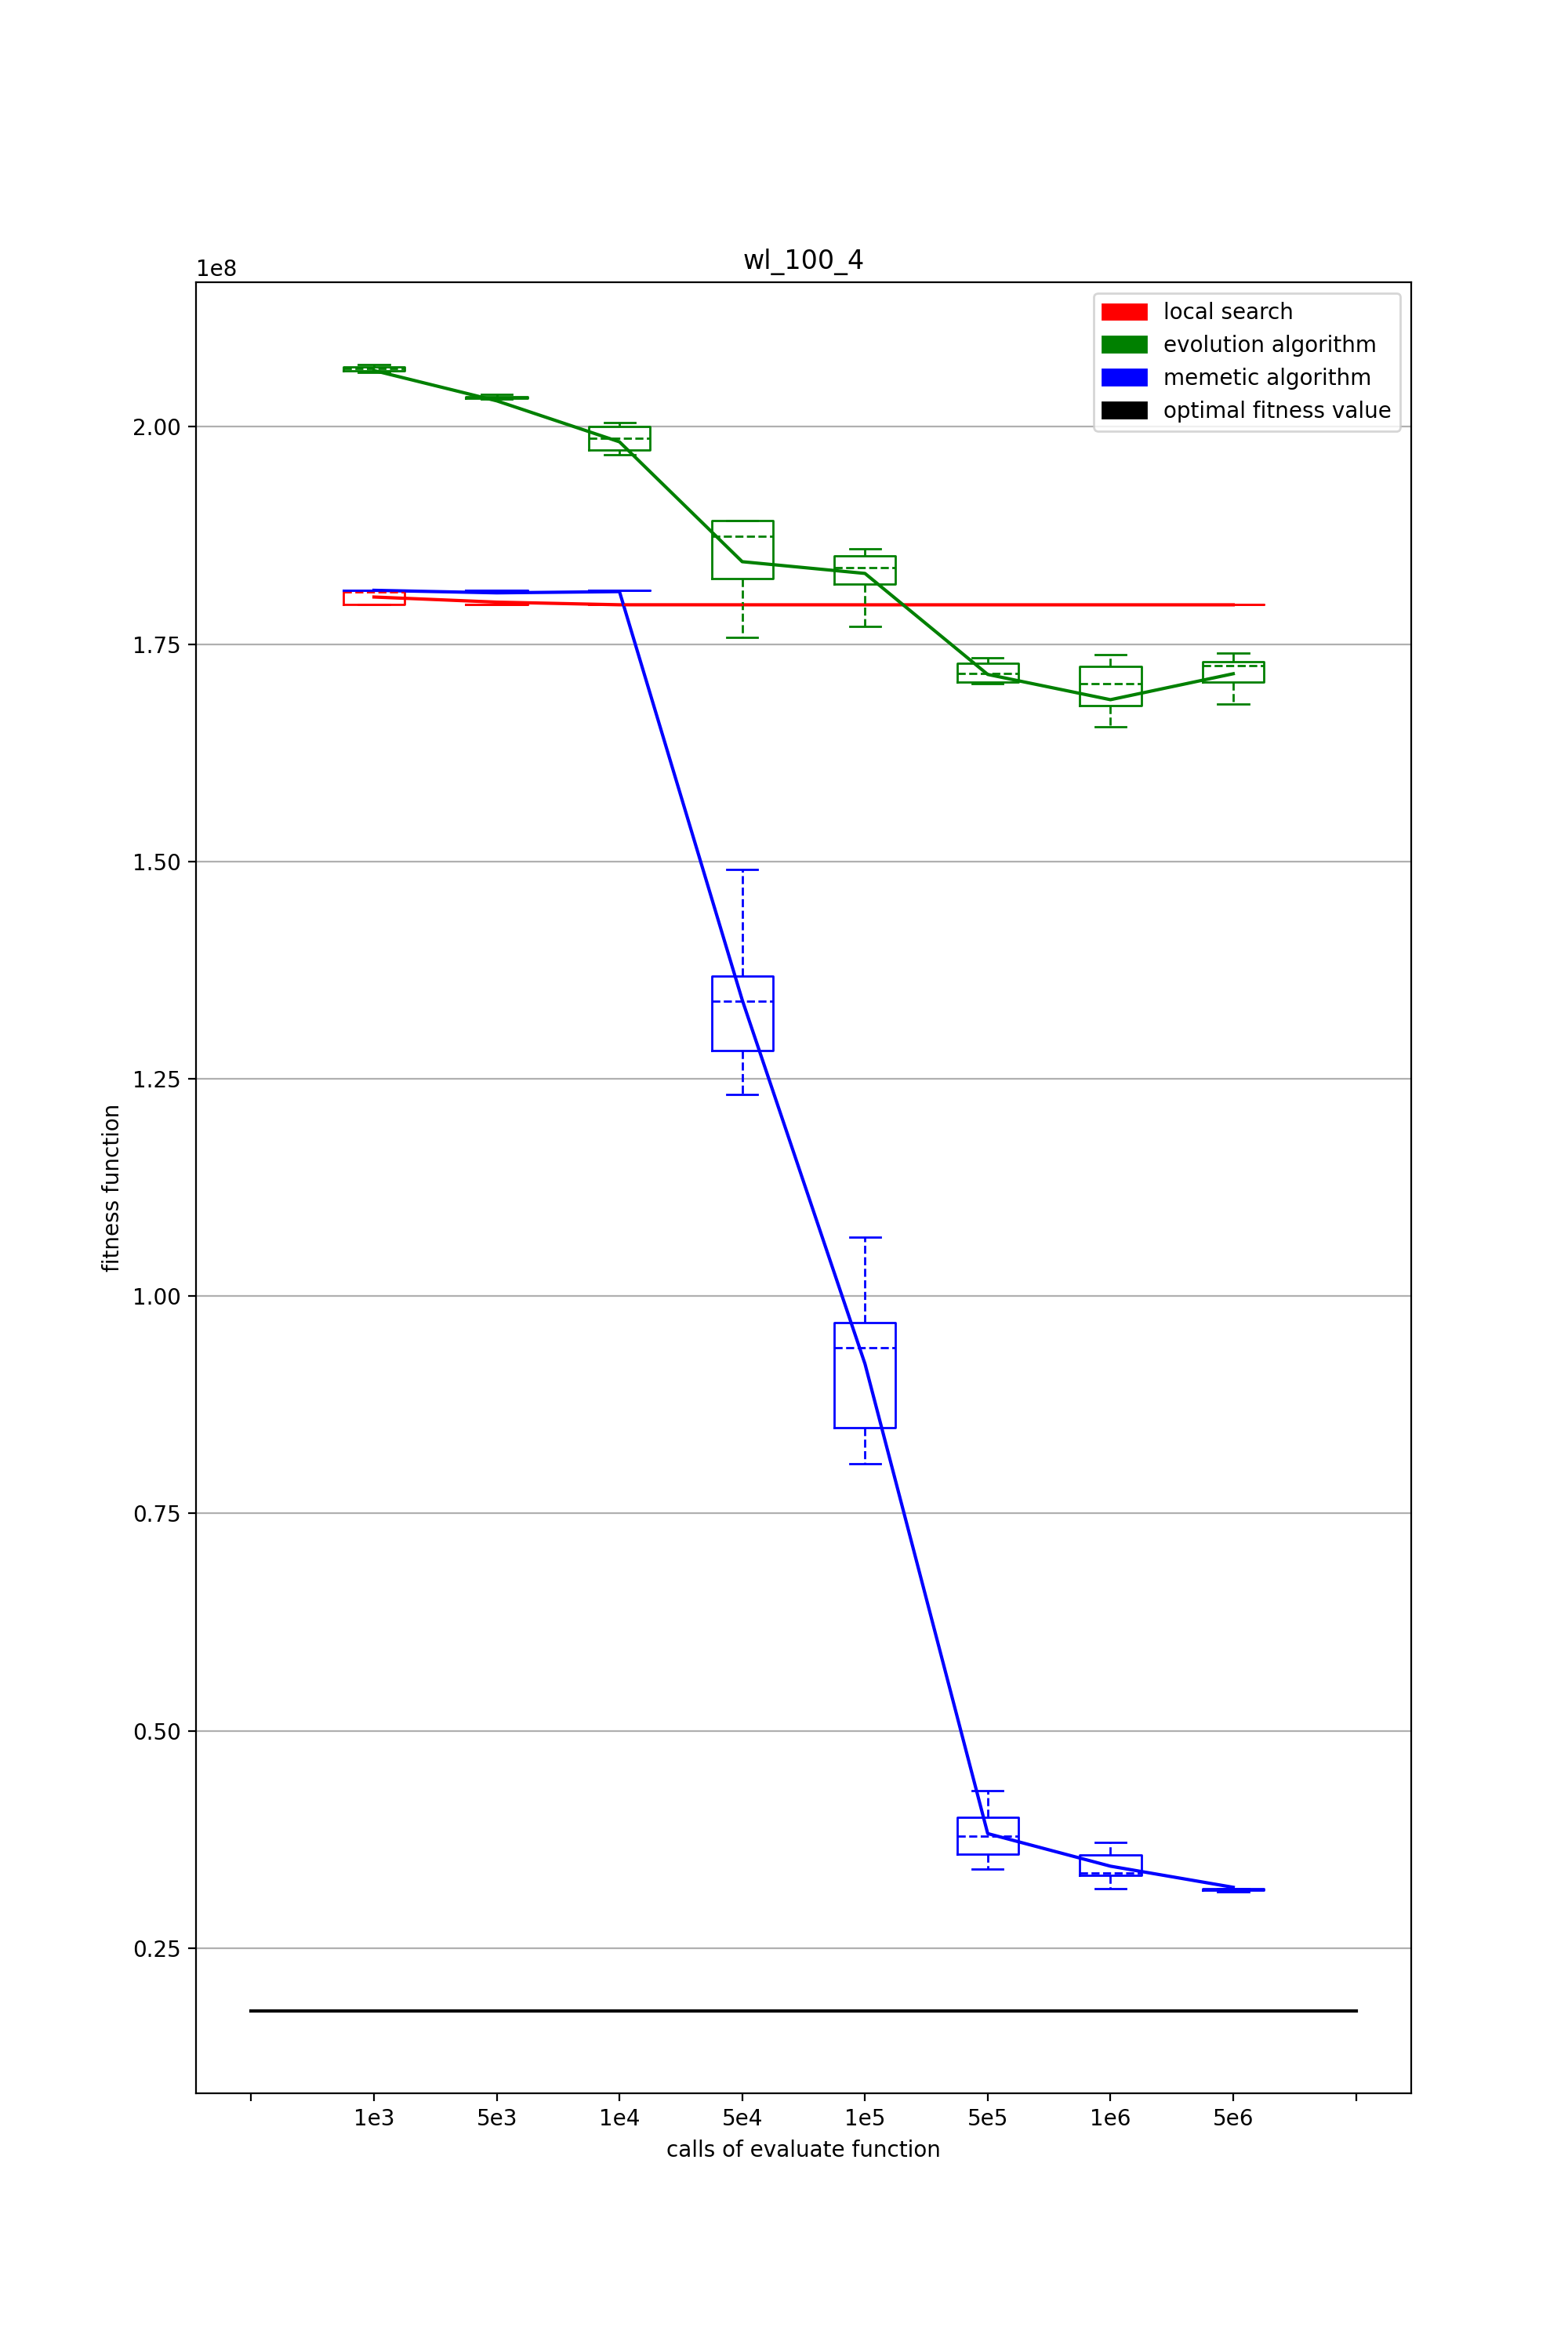
\includegraphics[width=0.6\linewidth]{wl_100_4.png}
    \caption{Comparison of algorithms on wl\_100\_4 instance}
\end{figure}

\newpage
\subsection{wl\_200\_1, wl\_500\_1, wl\_1000\_1, wl\_2000\_1}
On the remaining $4$ instances, the situation is almost the same.

On every number of evaluation calls evolution algorithm is much better than local search.
Here, the search space is too large and the random mutation does not suffice to explore significant portion of it.
It converges, but really slowly.

The evolution algorithm has a big jump in the first evaluation limits, but then it does not improve much.
The population probably starts to stagnate and then the case is the same as with local search.
It improves slightly, but it is not fast enough.

The memetic algorithm shows its power here.
It starts really bad, because it wastes evaluation function calls on local search, but it improves gradually with increasing the limit and after approximately $100 000$ evaluations, it takes over both local search and evoluion algorithm.
Also its confidence bounds are tight, so very similar solution is found almost every time.
It cannot be seen very well from the plot, but the bsf solutions of evolution and memetic algorithms are quite far away.
\begin{figure}
    \centering
    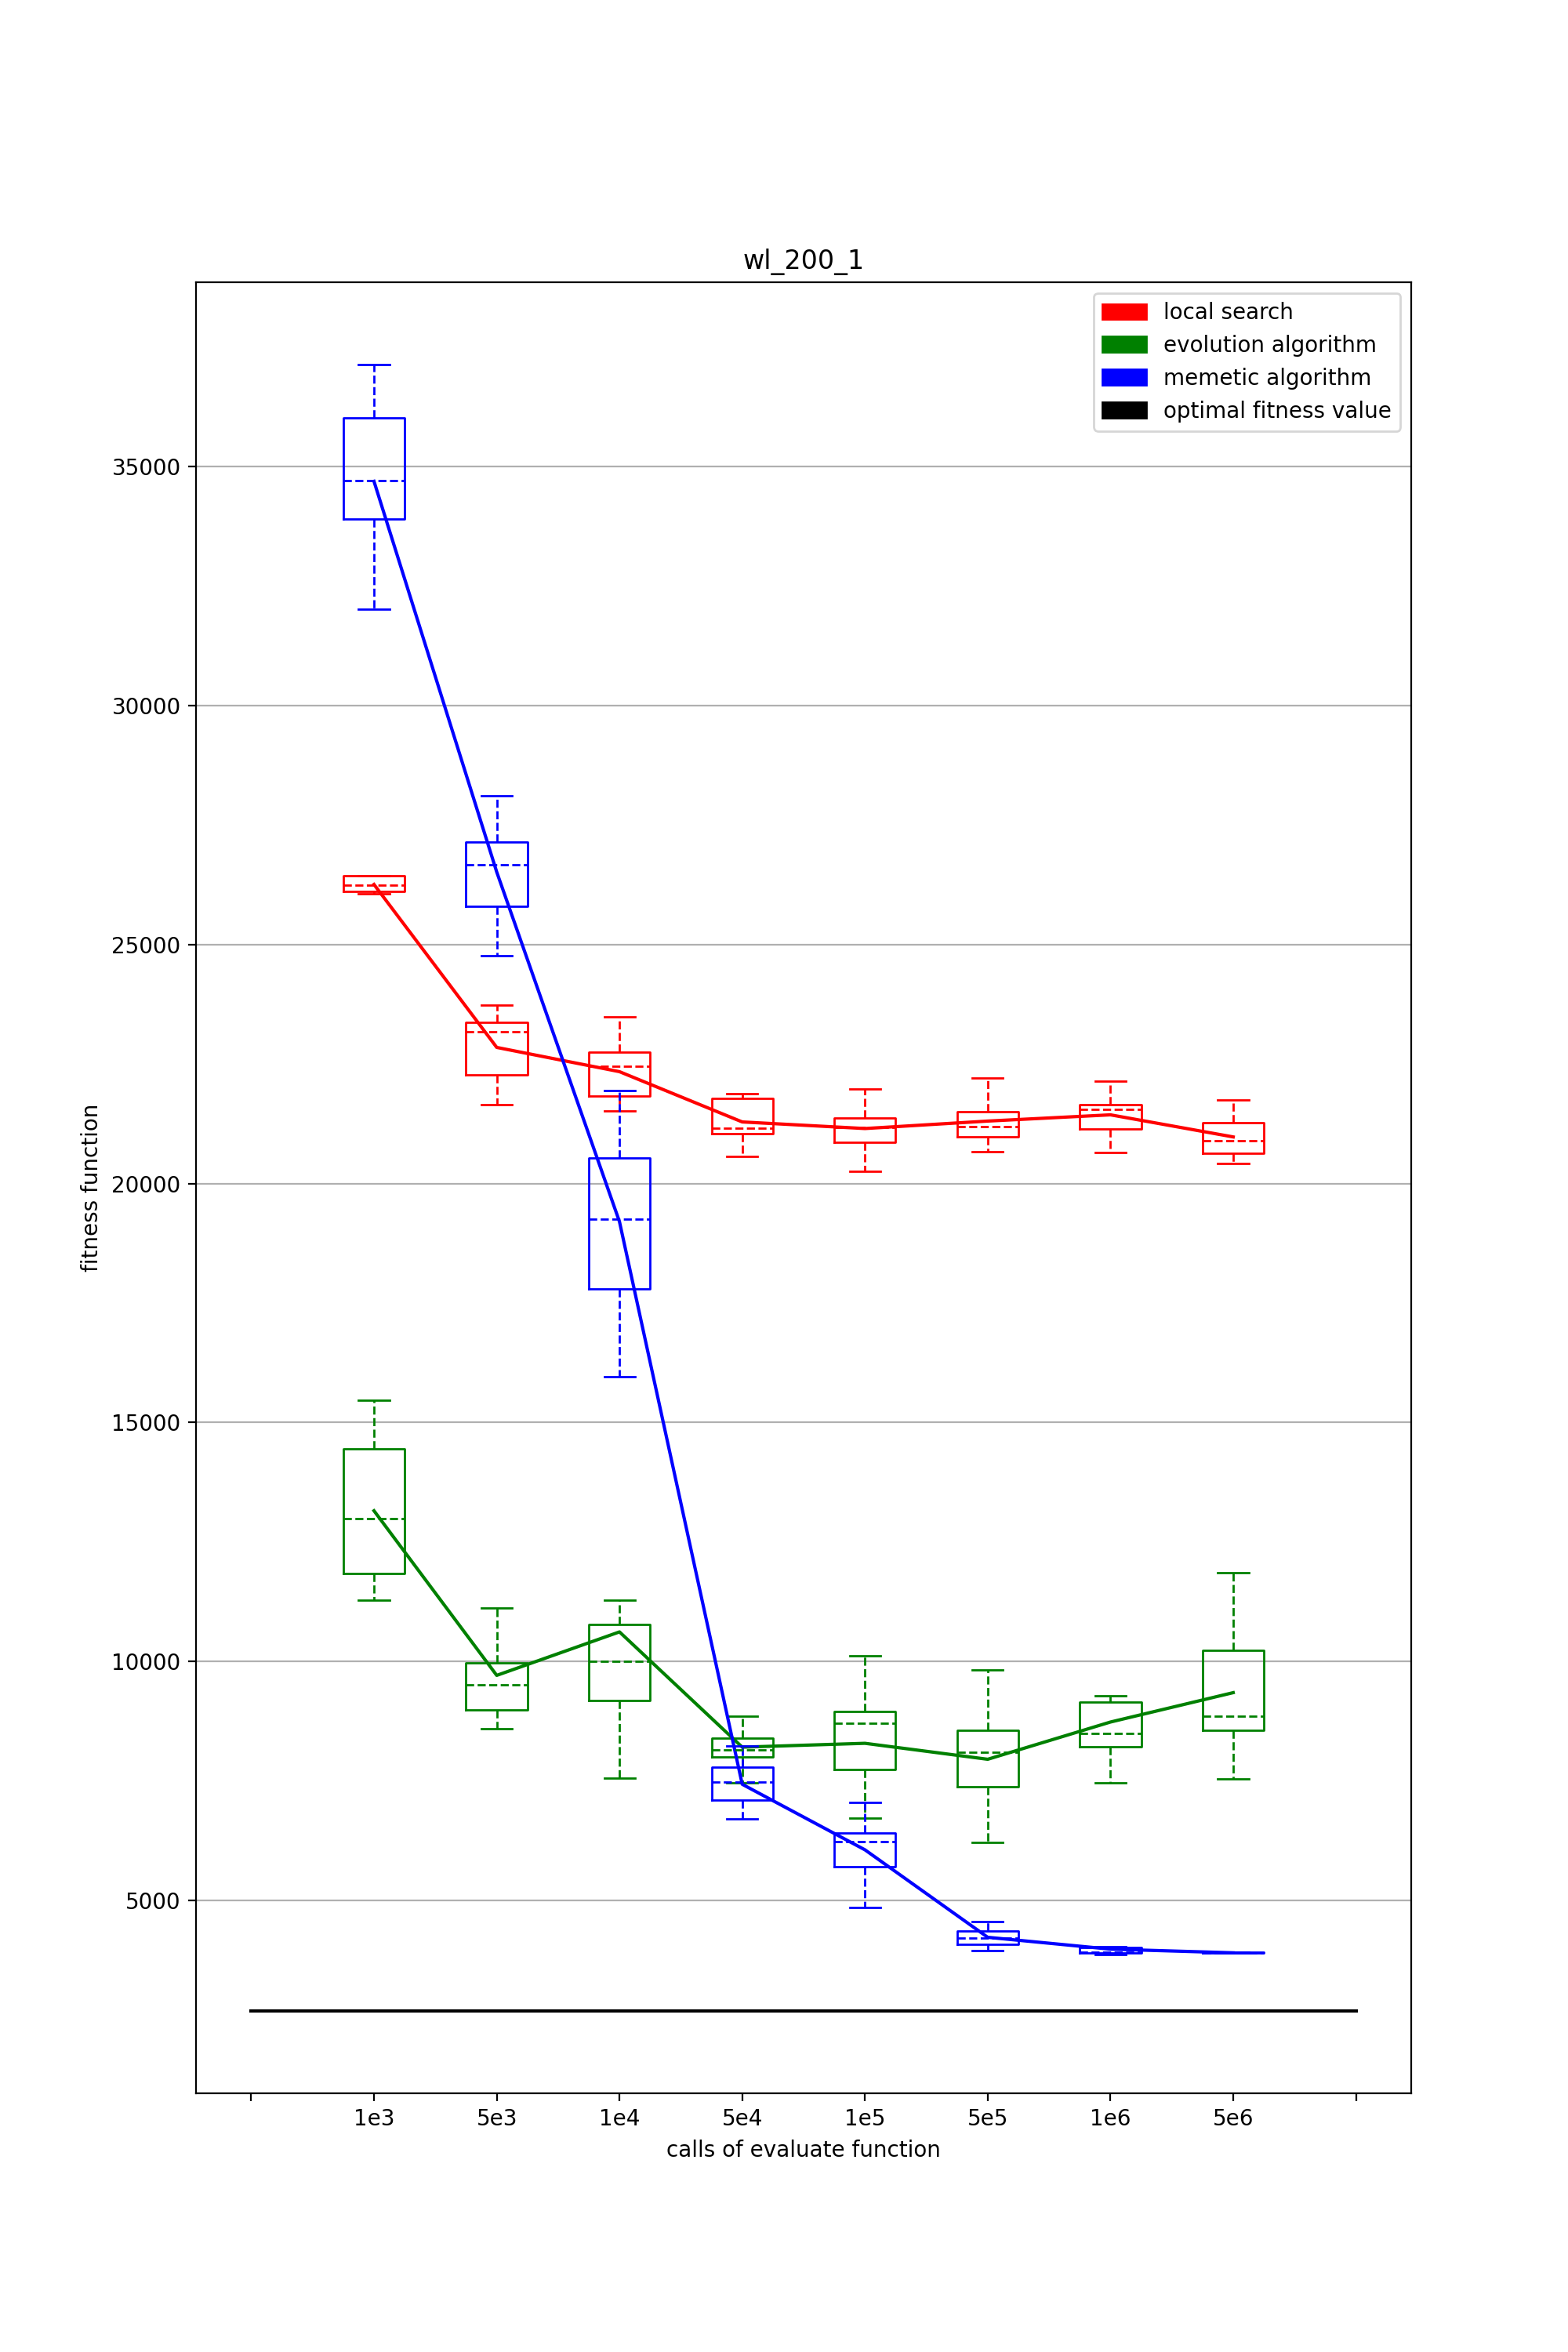
\includegraphics[width=0.6\linewidth]{wl_200_1.png}
    \caption{Comparison of algorithms on wl\_200\_1 instance}
\end{figure}
\begin{figure}
    \centering
    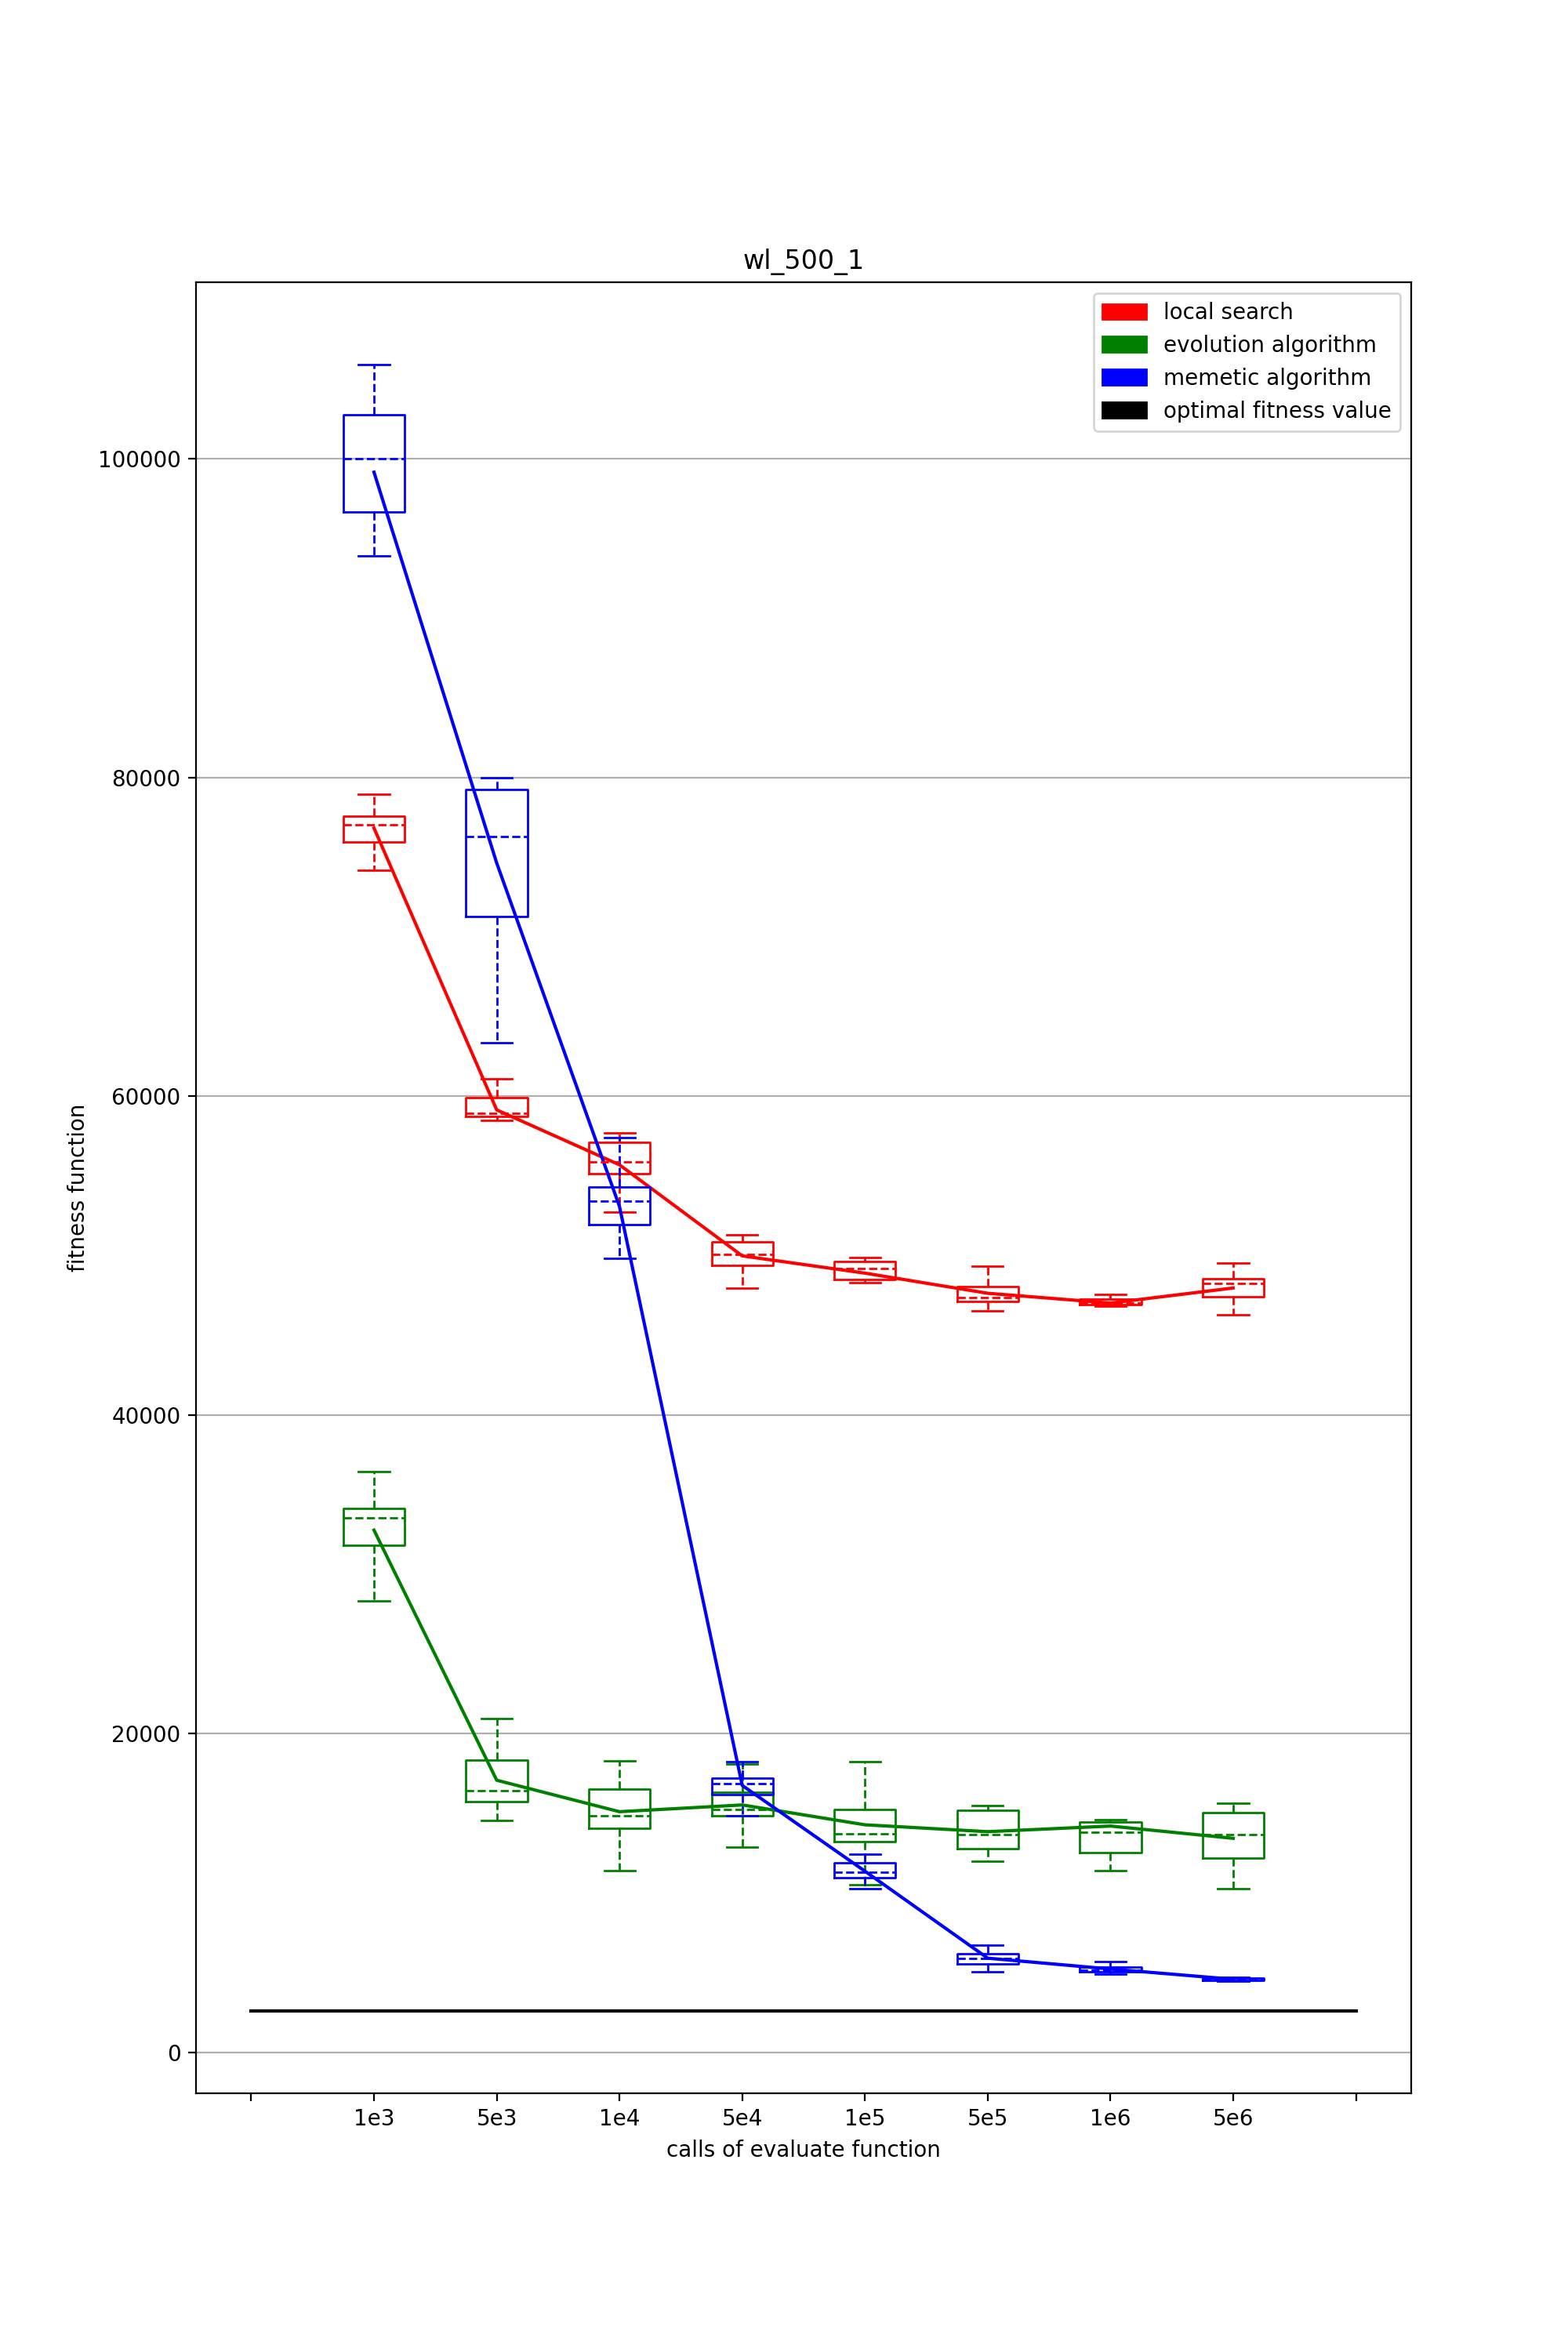
\includegraphics[width=0.6\linewidth]{wl_500_1.png}
    \caption{Comparison of algorithms on wl\_500\_1 instance}
\end{figure}
\begin{figure}
    \centering
    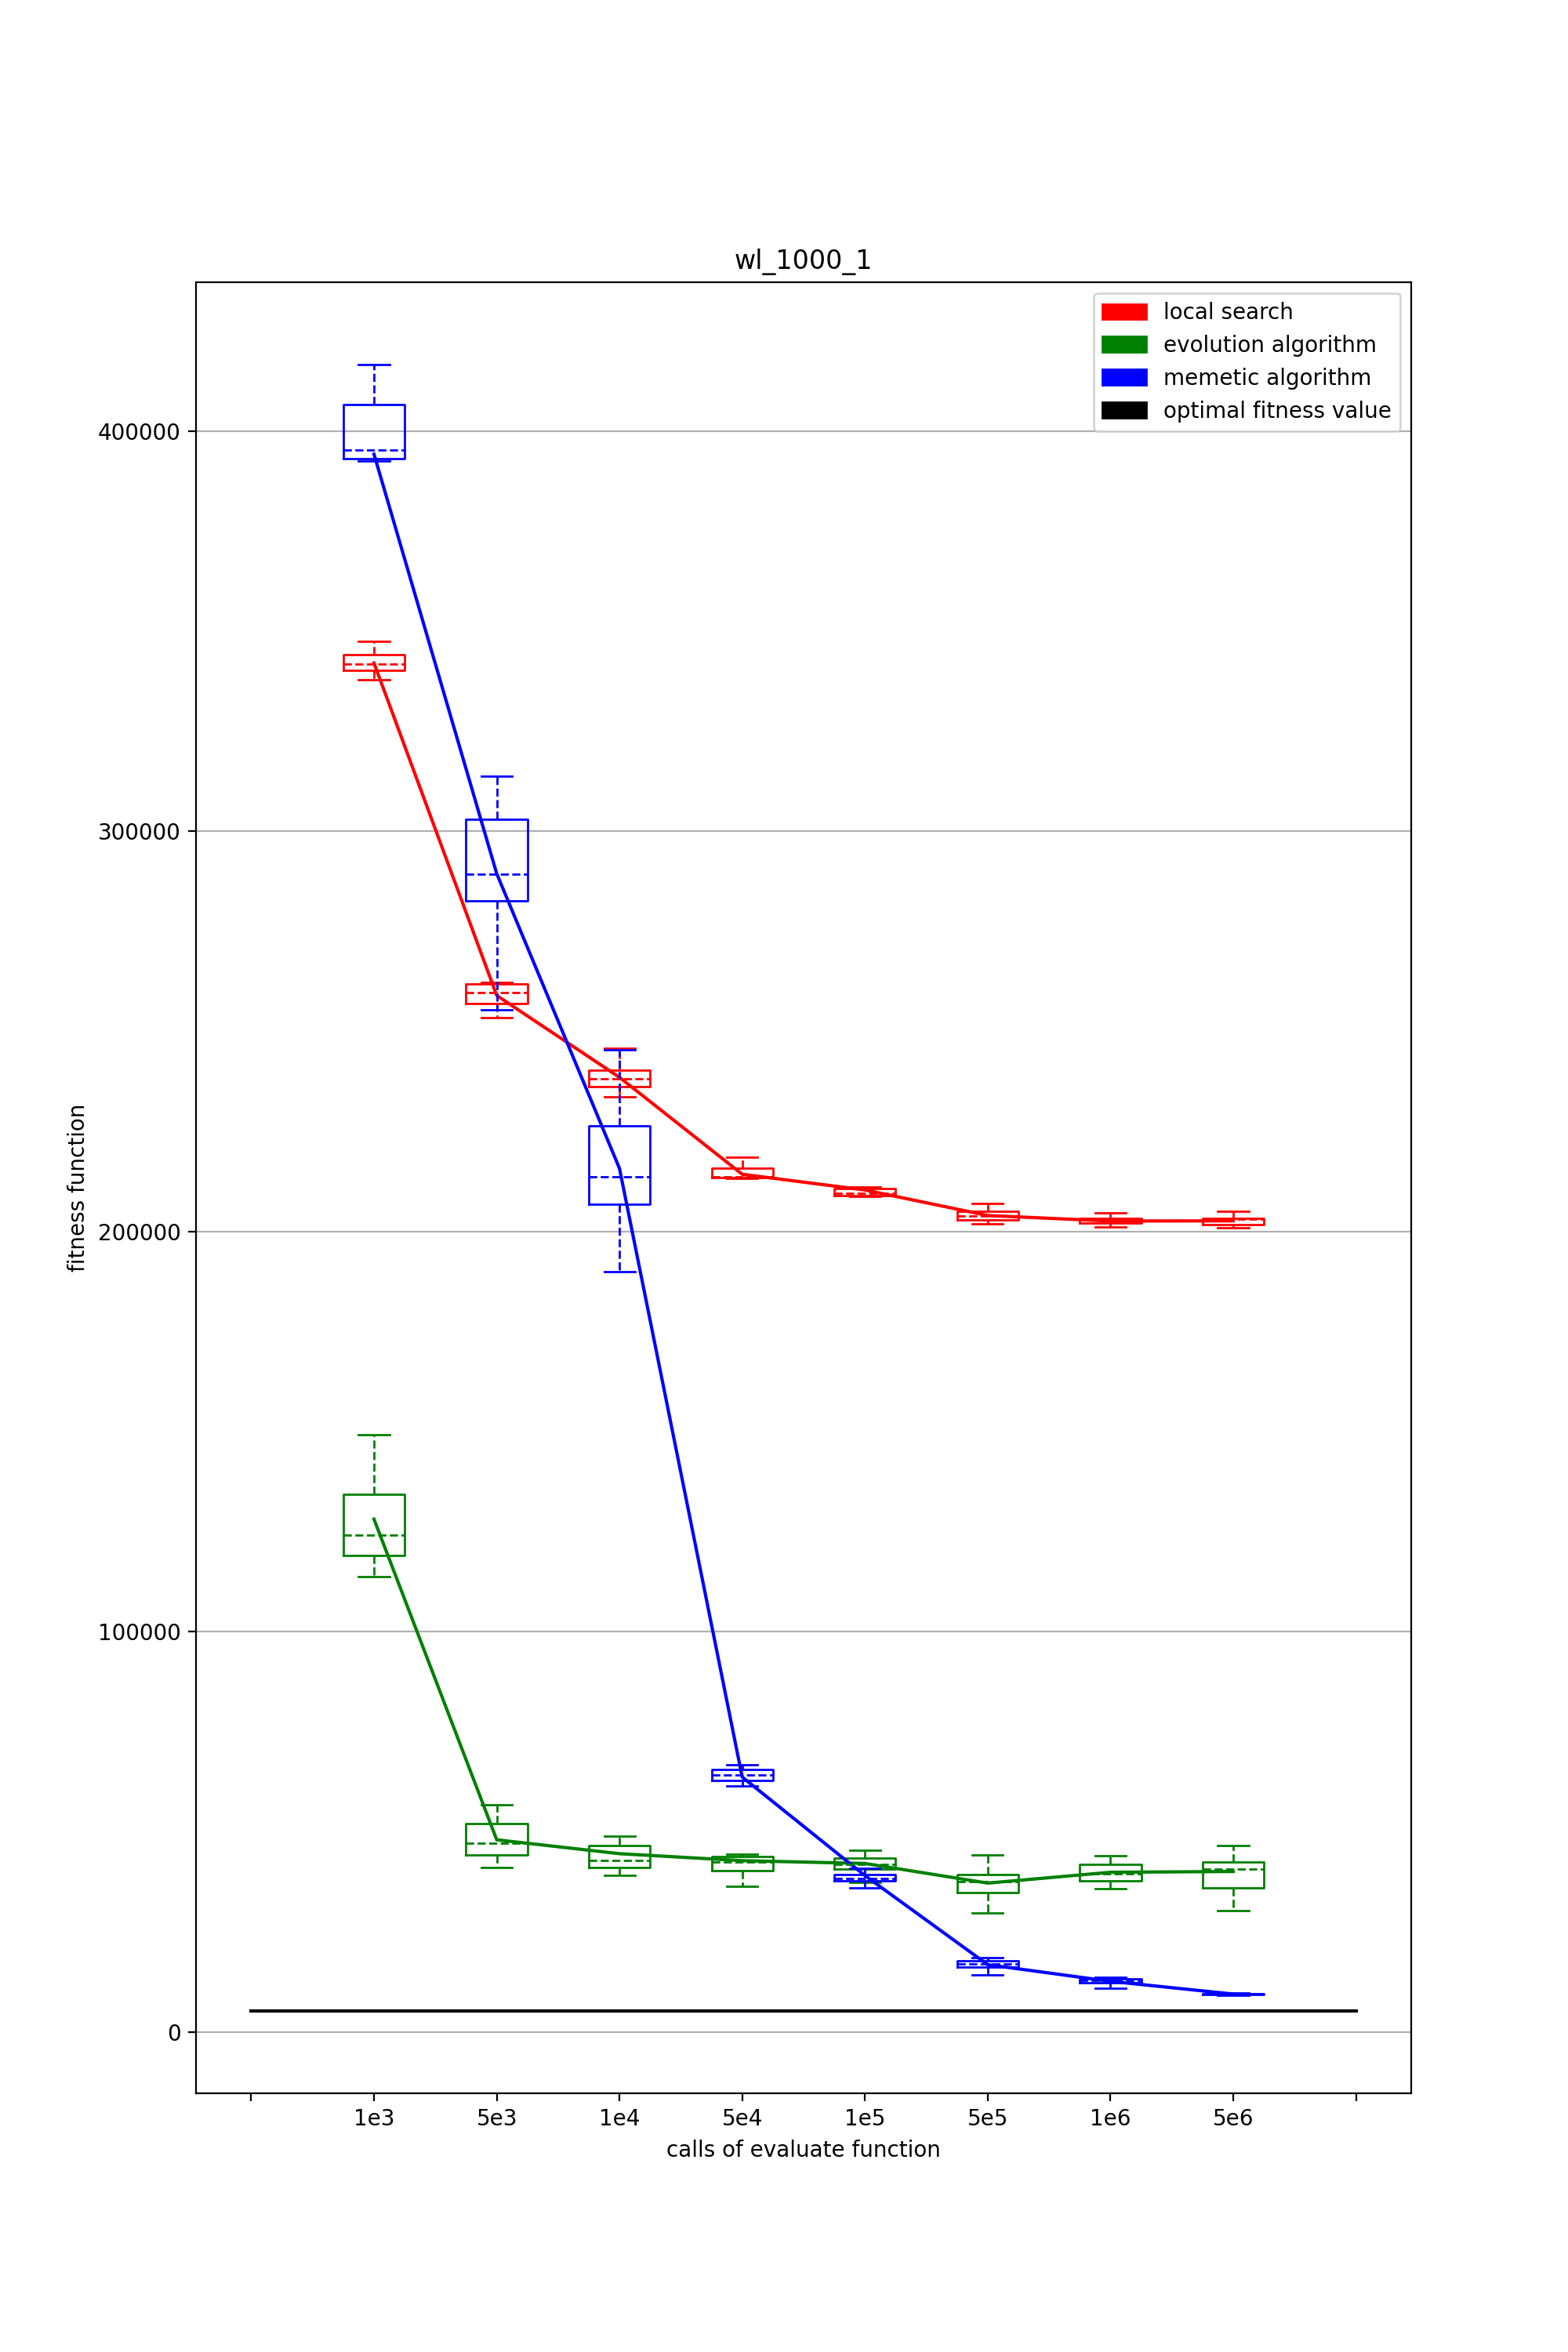
\includegraphics[width=0.6\linewidth]{wl_1000_1.png}
    \caption{Comparison of algorithms on wl\_1000\_1 instance}
\end{figure}
\begin{figure}
    \centering
    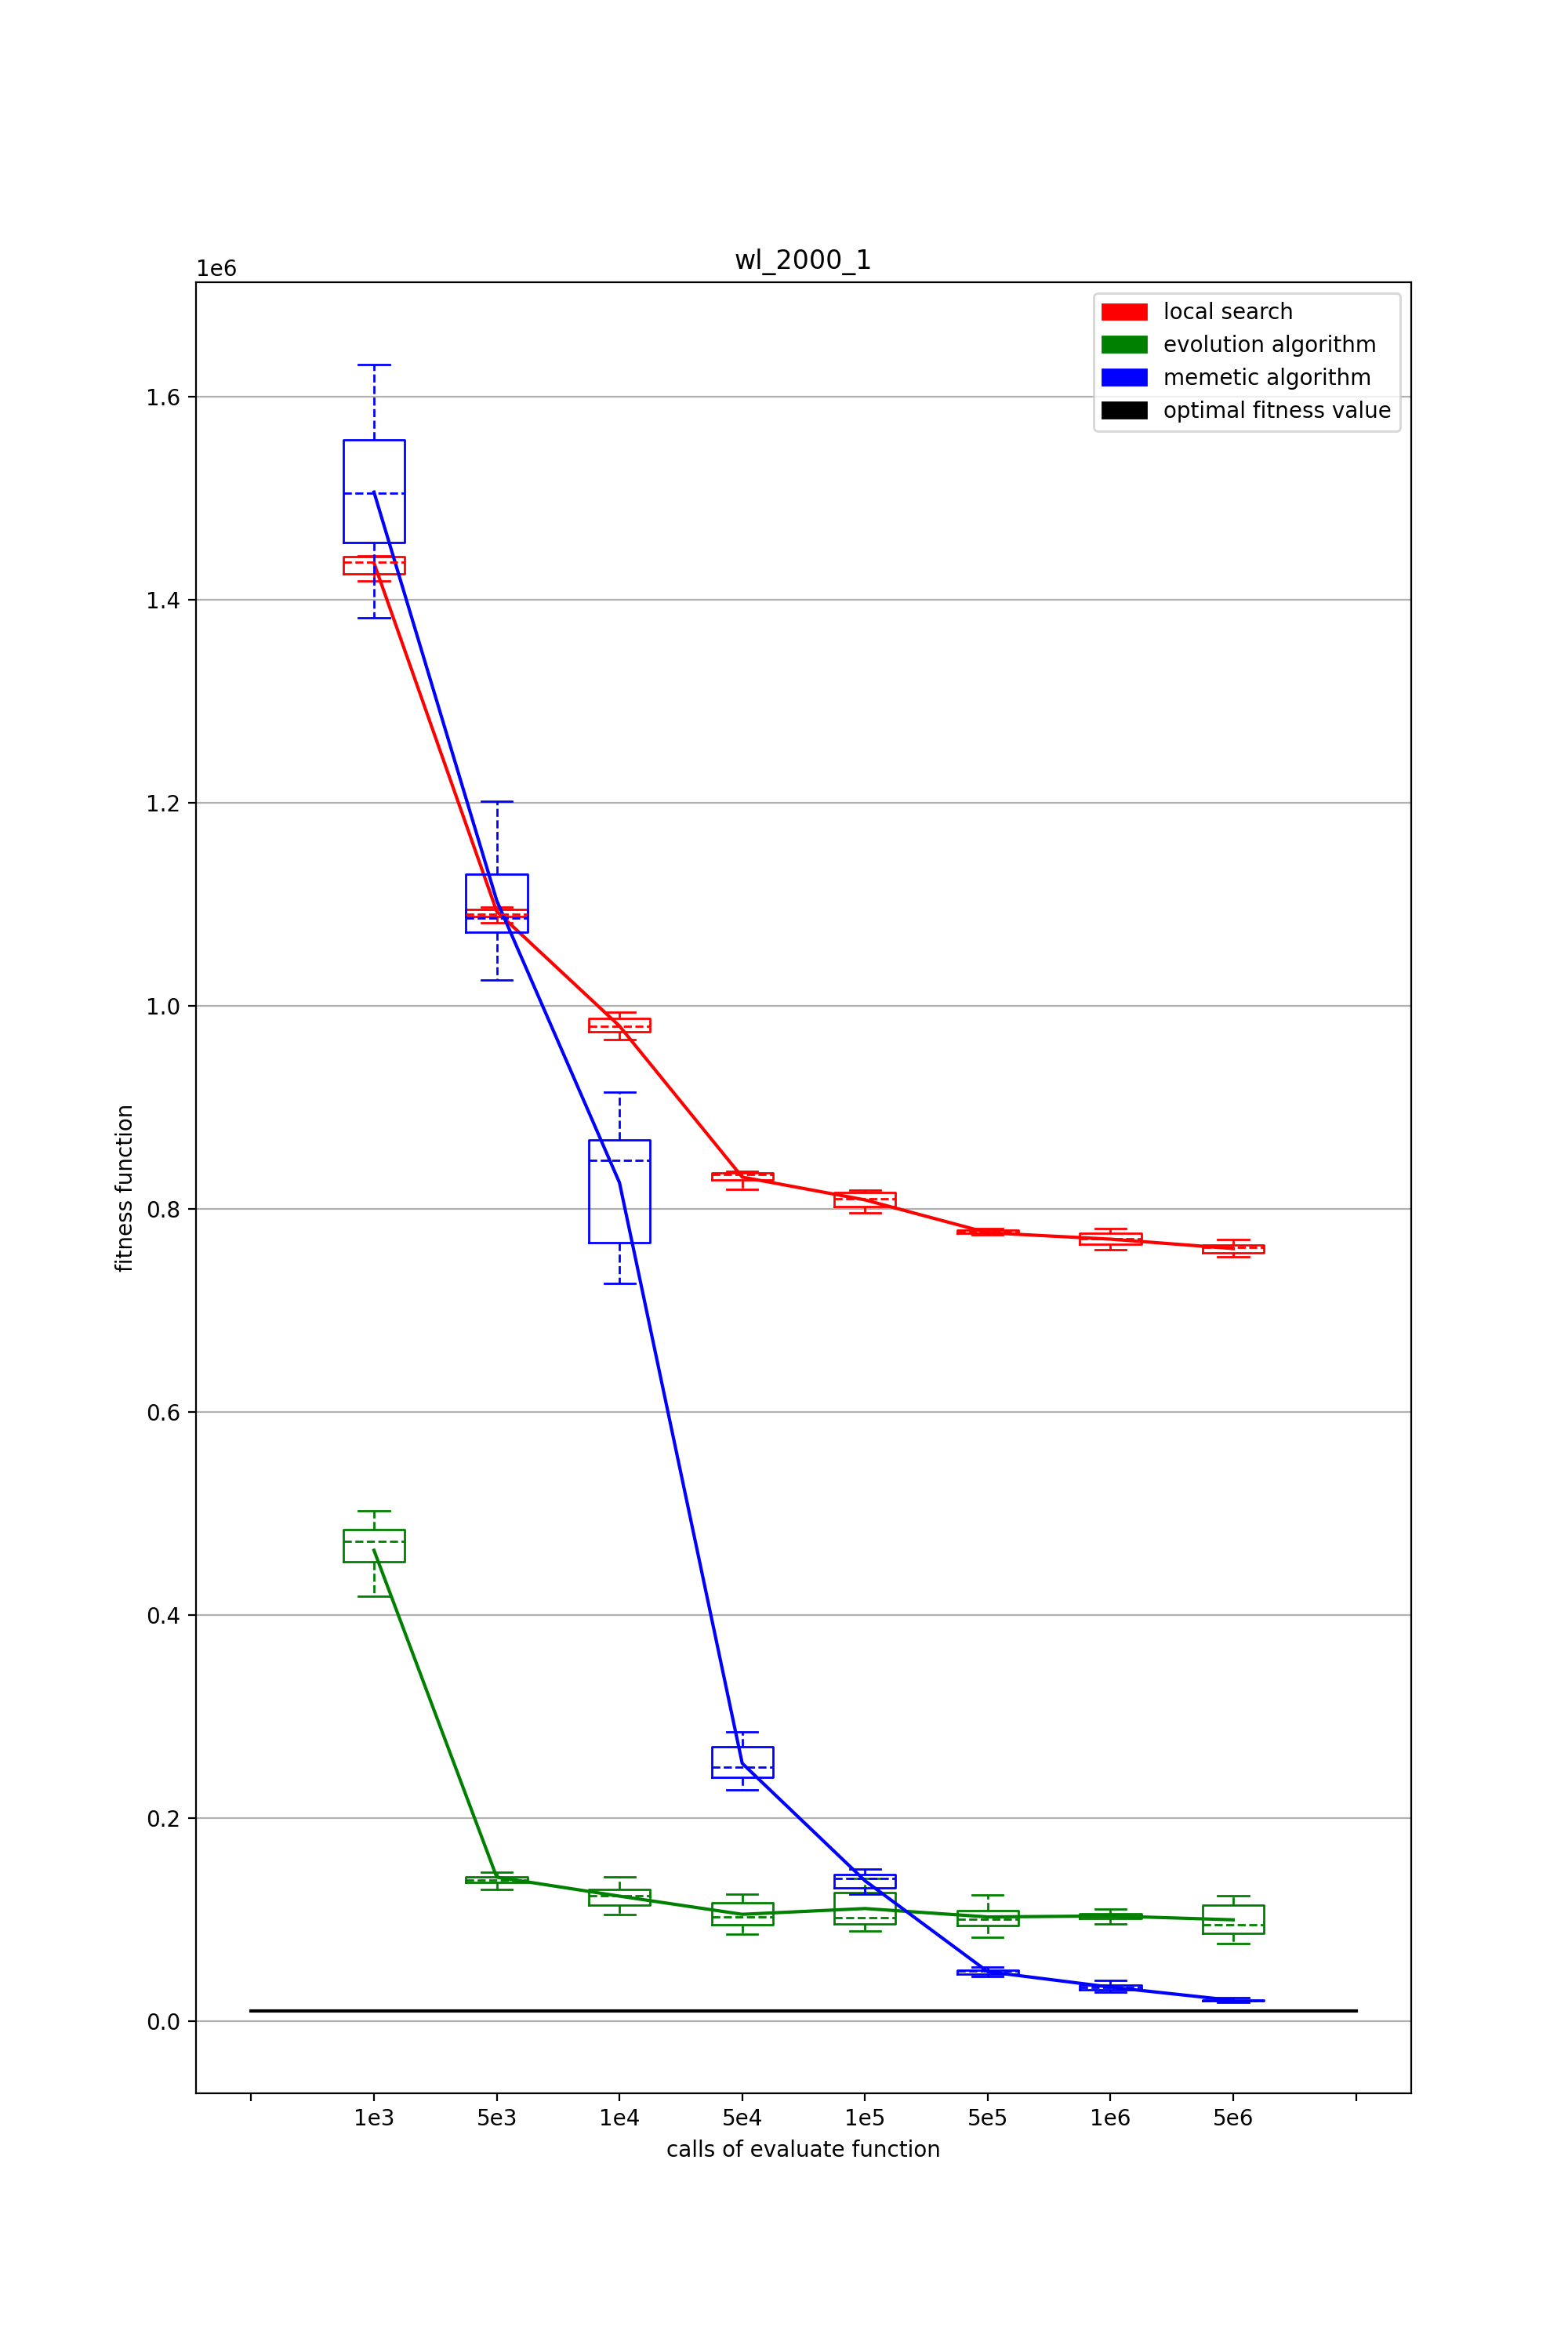
\includegraphics[width=0.6\linewidth]{wl_2000_1.png}
    \caption{Comparison of algorithms on wl\_2000\_1 instance}
\end{figure}

\end{document}

